\documentclass[10pt, a4paper,english,spanish,hidelinks]{article}
\usepackage{amsmath}
\usepackage{amsfonts}
\usepackage{amssymb}
\usepackage{caratula}
\usepackage[spanish, activeacute]{babel}
\usepackage[usenames,dvipsnames]{color}
\usepackage[width=15.5cm, left=3cm, top=2.5cm, height= 24.5cm]{geometry}
\usepackage{graphicx}
\usepackage[utf8]{inputenc}
\usepackage{listings}
\usepackage{multicol}
%\usepackage{subfig}
\usepackage{float}
\usepackage{color,hyperref}
\usepackage{listings}
\usepackage{caption}
\usepackage{subcaption}

\usepackage{listings}
\usepackage{babel}
\usepackage{url}
\usepackage{lscape}
\parindent = 15 pt
\parskip = 11 pt

\usepackage{fancyhdr}
\usepackage{hyperref}
\usepackage{amsmath}
\usepackage{amsfonts}
\usepackage{amssymb}
\usepackage[utf8]{inputenc}
\usepackage{graphicx}
\usepackage{caption}
\usepackage{color}
\usepackage{appendix}
\usepackage{fancyhdr}
\usepackage{graphicx}


\materia{Teoría de las Comunicaciones}

\titulo{Trabajo Práctico 1}
\fecha{29 de Abril de 2014}
\integrante{Gauder, Maria Lara}{027/10}{marialaraa@gmail.com}
\integrante{Kovacs, Ignacio Javier}{627/10}{ignacio.k91@gmail.com}
\integrante{Puerta, Armando Ezequiel}{812/09}{eze19.2009@gmail.com}
\integrante{Reartes, Marisol}{422/10}{mreartes5@gmail.com}

\begin{document}
\pagestyle{myheadings}
\maketitle
\markboth{Teoría de las Comunicaciones}{Wiretapping}

\thispagestyle{empty}
\tableofcontents
\newpage

%\centerline{\includegraphics[width=1\textwidth]{./graficos/entropia_juan_1.png}}

\section{Introducción}
EL objetivo principal del siguiente trabajo práctico consiste en observar distintas redes, mediante diferentes herramientas, y realizar un exhaustivo análisis a partir de la información obtenida. Las herramientas utilizadas para poder escuchar y manipular los paquetes de la red son: Wireshark y Scapy. Una vez recolectada la información requerida de los paquetes de la red, se realizarán comparaciones y conclusiones a partir de lo observado. 

En la primera parte del trabajo práctico se definirá una fuente diferente a la dada por la cátedra, se calculará las probabilidades de ambas fuentes, y, en consecuencia, sus entropías. 

Luego, en la segunda mitad, se realizará un análisis que permita, para cuatro redes diferentes, definir los protocolos distinguidos, analizar el overhead impuesto por el protocolo ARP y, además, determinar los nodos distinguidos. 
\newpage
\section{Capturando tráfico}

\subsection{Desarrollo}

En primer lugar se implementó una herramienta que permita escuchar de forma pasiva a la red local. De esta manera, se podran obtener los paquetes ARP y Ethernet que se encuentran en la red. 

La herramienta está desarrollada utilizando el lenguaje Python y la herramienta Scapy. Para poder trabajar de una manera más cómoda, también se desarrolló un enterno gráfico que permite visualizar las tomas de paquetes que se estan realizando. El mismo fue implementado para PyQT4. También se permite realizar capturas durante un tiempo determinado (pausado por el usuario o intervalo definido al inicio de la ejecución) y almacenarlas luego.  
De los paquetes ARP que se obtienen de la red, se almacenan las direcciones IP tanto del receptor como del emisor del mismo. Además, se distingue de los paquetes que envían un \textit{Request}, de los que envían \textit{Replay}. En el caso de los paquetes de tipo Ethernet, se almacenan las direcciones MAC tanto del emisor como del receptor y, además, el campo type.

A su vez, mientras se realizan las capturas de los paquetes que se encuentren en determinada red, se realizarán los cálculos necesarios para poder obtener la entropía, de acuerdo a la fuente de información definida. De esta manera, procedemos a describir las dos fuentes de información, las cuales se utilizarán de base para el analisis del comportamiento de los nodos en la red. 

El primer modelo de fuente de información está dado por la cátedra y se define que la misma distingue a los protocolos que se encapsulan en todos los paquetes ethernet de una red específica. Cada símbolo se diferenciará del otro a partir del valor del campo type del frame de capa 2.

El segundo modelo de fuente de información se basa únicamente en los paquetes ARP que se encuentren en la red. Los paquetes son distinguidos a partir de los tres campos que poseen: la dirección IP del host fuente, la dirección IP del host de destino y si es de tipo Replay o Request. 
Al primer modelo lo llamaremos ``Modelo Ethernet'' y al segundo ``Modelo ARP''.

\subsection{Modelo ARP}
El modelo de fuente de información que se decidió plantear, consiste en tomar como evento al suceso ``el host fuente con ciertas direcciones IP envía un paquete al host destino con otras direcciones IP con un pedido de Request o Replay''. Por consiguiente, se toma como fuente los dispositivos que mandan paquetes diferenciandolos por el tipo de mensaje que envían.

Luego, para el cálculo de la entropía se almacena un diccionario que contiene como claves a los cinco que contienen los paquetes ARP. Por lo que, al llegar un nuevo evento, se incrementa en uno la cantidad de apariciones del mismo, o en caso de ser la primera vez de su ocurrencia, entonces se lo agrega al diccionario, iniciándolo en uno.

La probabilidad de que ocurra un evento en este modelo implica una relación entre la cantidad de paquetes capturados hasta ese momento por un símbolo determinado contra la cantidad total de paquetes ARP obtenidos hasta el momento. 
La cantidad de información contenida en un evento determinado se obtiene a partir del siguiente cálculo: 
\begin{equation}
 I(s) = -log_{2}(P(s))
\end{equation}
Siendo s un evento, y P(s) la probabilidad de que ocurra el mismo. 
Finalmente la entropía de una fuente se calcula de la siguiente manera: 
\begin{equation}
 H(S) = \sum_{s \in S} P(s) I(s)
\end{equation}
Se utiliza el logaritmo en base dos, ya que la información se representa mediante bits. A partir de la entropía se podrá proceder al análisis de la información obtenida.

\subsection{Modelo Ethernet}
El modelo de fuente de información planteado por la cátedra implica distinguir a los paquetes por lo que indiquen en el campo type. Se distinguirán de esta manera a los nodos por el tipo sin importar quien es el host emisor y quien es el receptor. 

Entonces, para el cálculo de la probabilidad de la aparición de cada símbolo de la fuente se almacena, para cada type, la cantidad de ocurrencias del mismo.

Luego, se aplica el mismo procedimiento que en el modelo anterior para el cálculo de la entropía.
\newpage
\section{Gráficos y análisis}
Para probar la herramienta desarrollada en la primera parte, se analizaron cuatro redes diferentes a partir de las dos fuentes de información, el Modelo Ethernet y el Modelo ARP. 
A continuación se presentan las cuatro LANs analizadas y sus correspondientes resultados. 

\subsection{Digrafos de las redes}\label{"Grafos"}

\subsubsection{Red Hogareña}
Como lo indica su nombre, la misma fue tomada en la casa de uno de los integrantes del grupo. Utilizandose la red Wifi se realizaron capturas de los paquetes Ethernet y, además, de los ARP, de acuerdo al modelo correspondiente. La red presentaba pocos dispositivos conectados y enviando y recibiendo información, por lo que permite un mejor análisis del comportamiento de la misma. 

A continuación se presenta un digrafo que muestra el comportamiento de la red para el Modelo ARP. Se presentan en los nodos a los dispositivos con su correspondiente dirección IP y las aristas corresponden a la cantidad de paquetes de tipo Replay o Request que ocurren entre dos host. 


\centerline{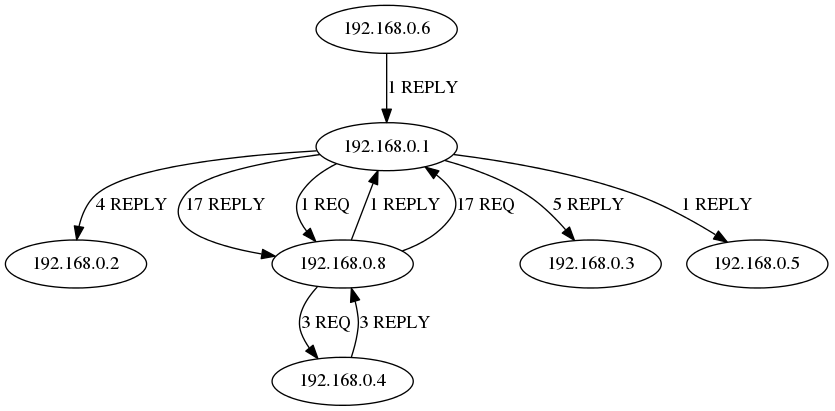
\includegraphics[width=1\textwidth]{./graficos/grafos-arp/grafo_casa_mari.png}}


Como se puede observar, el host con dirección IP 192.168.0.1 se podría comprender que consiste en el router, ya que es el capaz de responder con un mensaje de tipo Replay a todos los mensajes de tipo Request enviados. Luego, en secciones siguientes se podrá distinguir de manera clara cual representaría al nodo distinguido para el evento del Modelo ARP. 

\subsubsection{Red Laboratorio}
En este caso se decidió capturar los paquetes que se encontraban en la red cableada de uno de los laboratorios de la facultad. La cantidad de host que se encuentran interviniendo en la misma es mucho mayor a la de una red hogareña. Se muestra, a continuación, el digrafo generado a partir del evento "una dirección IP participa en el envío de un paquete de tipo Replay o Request a otra dirección IP". 

%Debido al gran número de dispositivos que se involucran en la red, se decidió eliminar aquellos que únicamente participan en el recibimiento o envío de un solo paquete de tipo ARP. Ese filtro se aplica únicamente para la presentación del digrafo del evento "una dirección IP participa en el envío de un paquete de tipo Replay o Request a otra dirección IP".  

\centerline{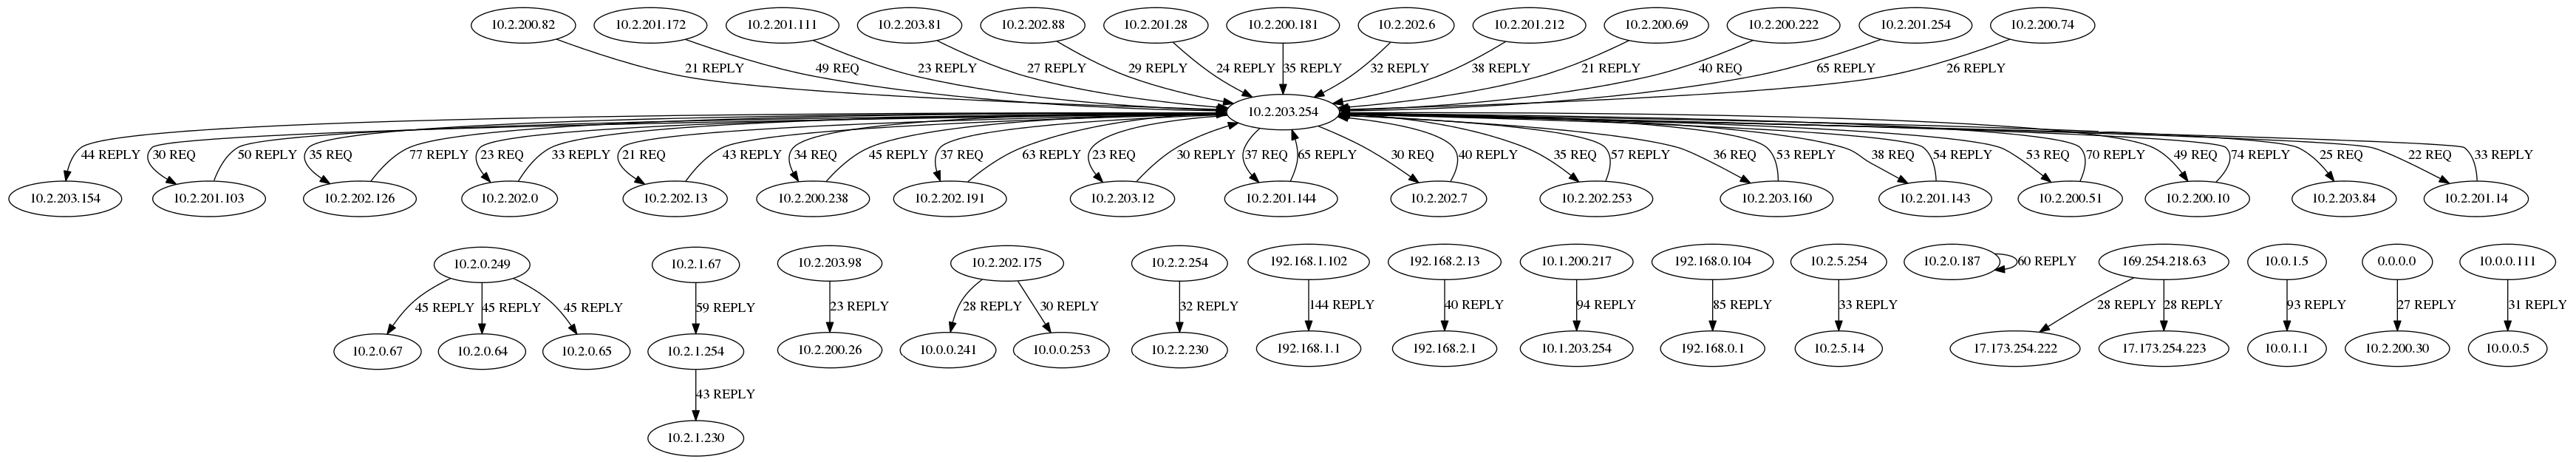
\includegraphics[angle=90, scale=0.3]{./graficos/grafos-arp/grafo_labo5.png}}

A partir del digrafo, se podría concluir que el nodo 10.2.203.254 es un nodo característico debido a la cantidad de información que posee. Luego, mediante otro tipo de análisis, se podrá definir de manera más clara, cual es el nodo característico correspondiente a esa fuente de información para la Red del Laboratorio. 


\subsubsection{Red Devartis}
Otra de las capturas se realizó en el trabajo de uno de los integrantes. Los paquetes se capturaron en la red cableada del lugar. Esta red cuenta con aproximadamente 16 host, 1 router y 1 servidor. Es decir, la red presenta un tamaño intermedio con respecto a las dos anteriores. Por lo que es más compleja de analizar que la red hogareña, pero mucho más simple que la red del laboratorio de la facultad. 
Debajo, se puede observar el digrafo obtenido. El mismo fue originado a partir del mismo evento que los anteriores. 

\centerline{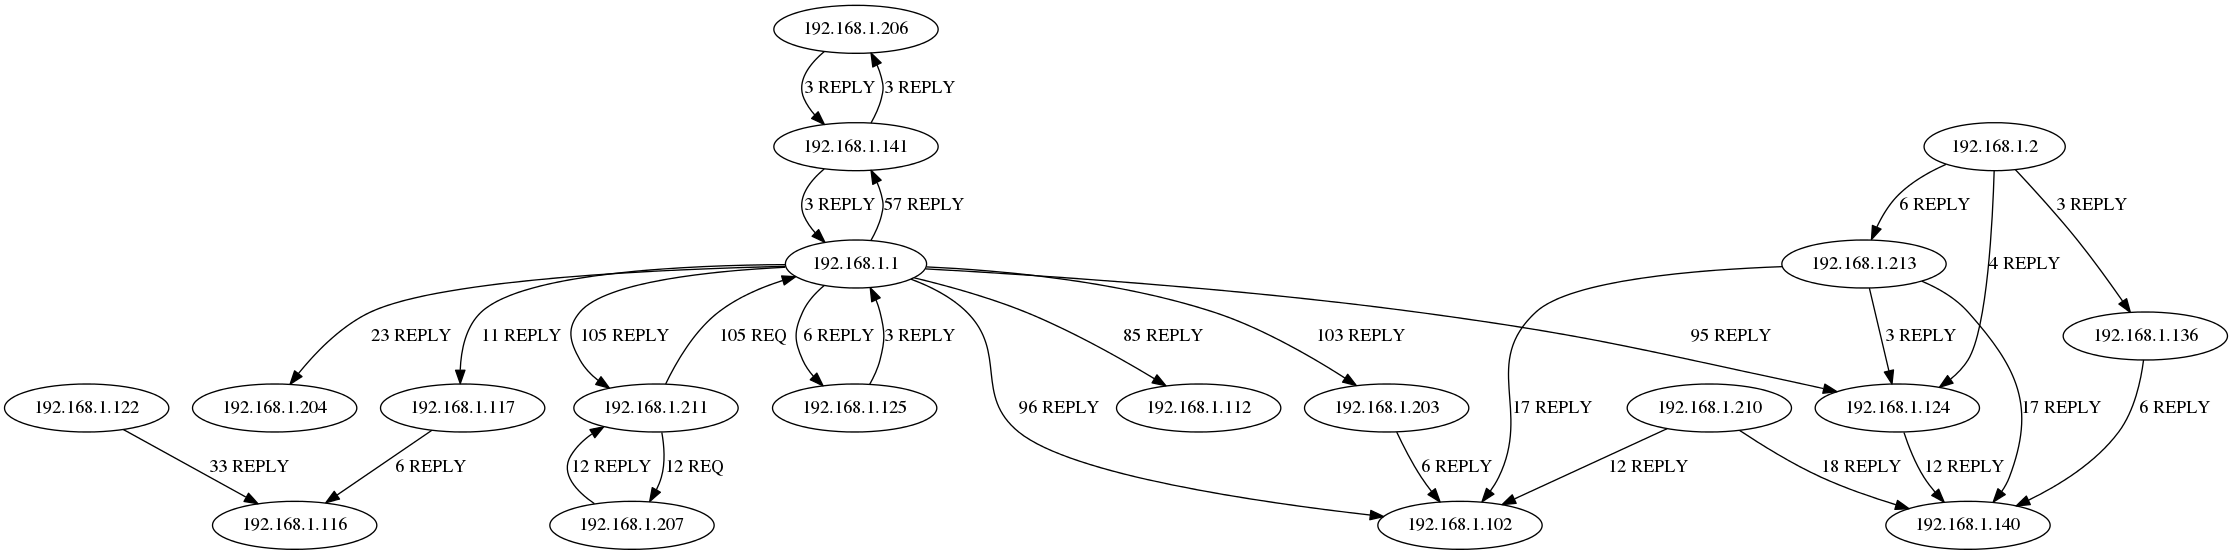
\includegraphics[angle=90, scale=0.3]{./graficos/grafos-arp/grafo_laburo_mari.png}}

Observando el grafo presentado, se puede notar que el nodo 192.168.1.1 es distinguido, por la cantidad de mensajes de tipo Replay que salen de mismo. Probablemente, la IP del nodo corresponda al router de la red. Esta  deducción, se podrá comprobar en el análisis de siguientes gráficos.

\subsubsection{Red Mercap}
Finalmente, la cuarta captura se realizó en el trabajo de otro de los integrantes. La red fue analizada desde una máquina virtual corriendo un sistema Linux, sobre un host Windows. Cabe aclarar que la misma estaba conectada a la red de manera física y que cuenta de 30 computadoras, 5 servidores y 1 router WiFi (además de los posibles dispositivos móviles conectados a la red de manera inalámbrica).

La captura duró una hora, durante la cual se obtuvo una enorme cantidad de relaciones generadas entre los diferentes actores, enviando y recibiendo los respectivos paquetes ARP. Esto ya aseguraba que el digrafo resultante (en primer instancia) iba a ser ilegible, aún ampliando la imagen (como observamos en el círculo con zoom sobre uno de los tantos nodos distinguidos de la red). 

\centerline{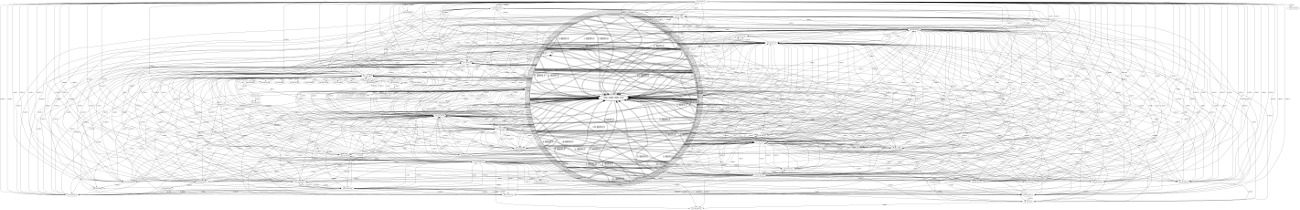
\includegraphics[angle=0,scale=0.3]{./graficos/grafos-arp/grafo_laburo_eze1.png}}

Es por eso que para analizar mejor la red y la interacción por medio de paquetes, decidimos mostrar solo aquellas relaciones en las cuales se envíen o reciban mas de 20 paquetes ARP. Este filtro solo se aplica para favorecer la visualización de los datos y de ninguna manera alteramos los resultados de la captura para los experimentos posteriores. De esta manera, observamos que la presente red toma un tamaño mucho mas manejable. Limitando la cantidad de nodos a mostrar, nos podemos concentrar en ver los nodos que realmente se destacan.

A simple vista observamos que los nodos 192.168.168.1, 192.168.168.2, 192.168.168.4, 192.168.168.36 y 192.168.168.135 concentran gran parte del intercambio de mensajes ARP de este segmento de la captura. De estos nodos distinguidos, en particular podemos inferir que los que tienen IPs mas bajas, probablemente sean algunos de los servidores de los que dispone la empresa. Potencialmente, los mas antiguos y utilizados, a saber; un servidor para Envy (control de versiones orientado a objetos - Smalltalk), un servidor que aloja la web empresarial, un CVS y otras herramientas como JIRA ó BambooHR (muy consultados a toda hora), y finalmente un servidor corriendo GemStone (base de datos no relacional).

\centerline{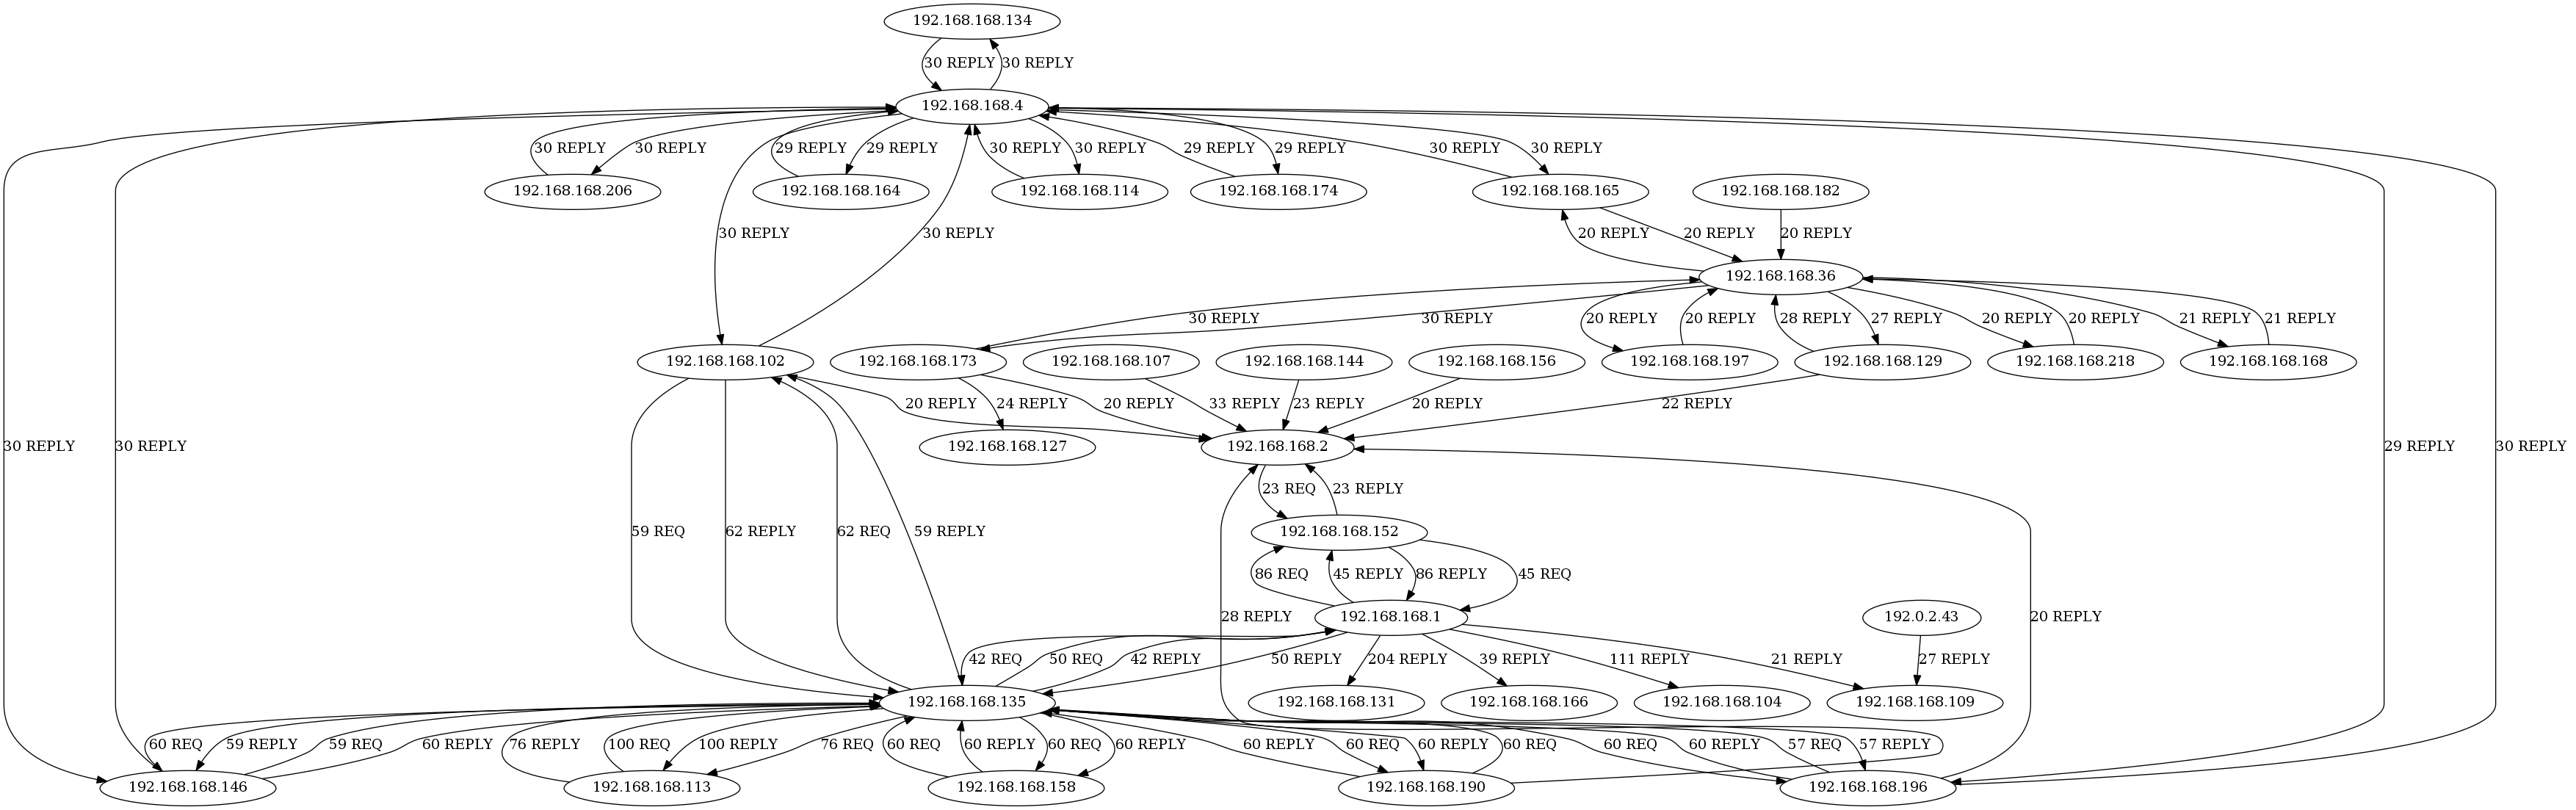
\includegraphics[angle=90,scale=0.2]{./graficos/grafos-arp/grafo_laburo_eze2.png}}
\newpage
\section{Gráficos y análisis}
Para probar la herramienta desarrollada en la primera parte, se analizaron cuatro redes diferentes a partir de las dos fuentes de información, el Modelo Ethernet y el Modelo ARP. 
A continuación se presentan las cuatro LANs analizadas y sus correspondientes resultados. 

\subsection{Digrafos de las redes}\label{"Grafos"}

\subsubsection{Red Hogareña}
Como lo indica su nombre, la misma fue tomada en la casa de uno de los integrantes del grupo. Utilizandose la red Wifi se realizaron capturas de los paquetes Ethernet y, además, de los ARP, de acuerdo al modelo correspondiente. La red presentaba pocos dispositivos conectados y enviando y recibiendo información, por lo que permite un mejor análisis del comportamiento de la misma. 

A continuación se presenta un digrafo que muestra el comportamiento de la red para el Modelo ARP. Se presentan en los nodos a los dispositivos con su correspondiente dirección IP y las aristas corresponden a la cantidad de paquetes de tipo Replay o Request que ocurren entre dos host. 

\begin{figure}{h!}{0.5\textwidth}
  \begin{center}
    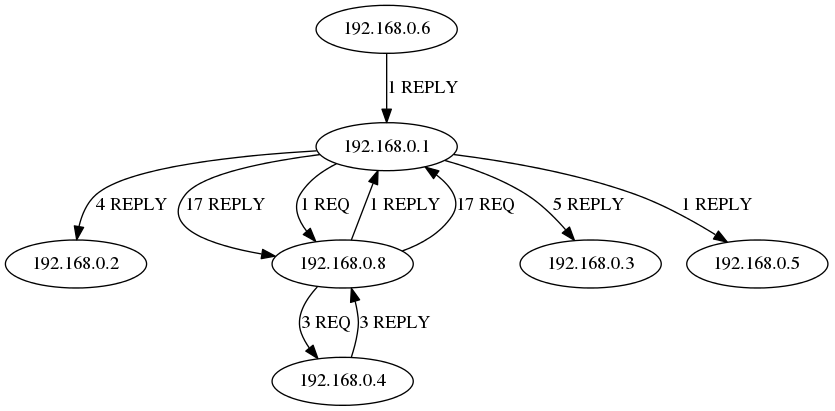
\includegraphics[width=1\textwidth]{./graficos/grafos-arp/grafo_casa_mari.png}
  \end{center}
  \caption{Digrafo: red hogareña}
\end{figure}

Como se puede observar, el host con dirección IP 192.168.0.1 se podría inferir que es el router, ya que es el capaz de responder con un mensaje de tipo Replay a todos los mensajes de tipo Request enviados. Luego, en secciones siguientes se podrá distinguir de manera clara cual representaría al nodo distinguido para el evento del Modelo ARP. 

\subsubsection{Red Laboratorio}
En este caso se decidió capturar los paquetes que se encontraban en la red cableada de uno de los laboratorios de la facultad. La cantidad de host que se encuentran interviniendo en la misma es mucho mayor a la de una red hogareña. Se muestra, a continuación, el digrafo generado a partir del evento ``una dirección IP participa en el envío de un paquete de tipo Replay o Request a otra dirección IP''. 

Debido al gran número de dispositivos que se involucran en la red, se decidió eliminar aquellos que únicamente participan en el recibimiento o envío de un solo paquete de tipo ARP. Ese filtro se aplica únicamente para la presentación del digrafo del evento ``una dirección IP participa en el envío de un paquete de tipo Replay o Request a otra dirección IP''.

\begin{figure}{h!}{0.5\textwidth}
  \begin{center}
    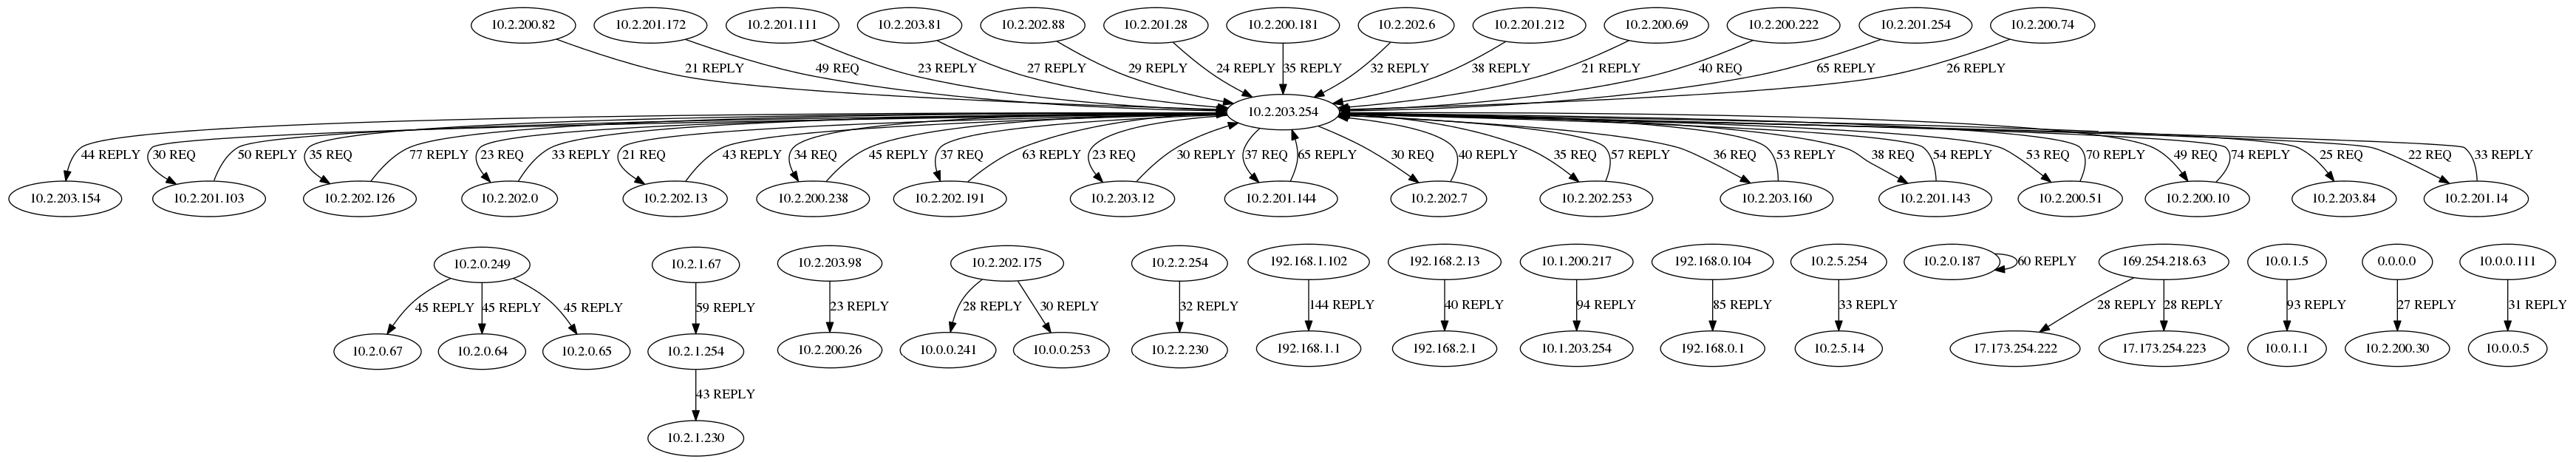
\includegraphics[angle=90, scale=0.3]{./graficos/grafos-arp/grafo_labo5.png}
  \end{center}
  \caption{Digrafo: red laboratorio}
\end{figure}

A partir del digrafo, se podría concluir que el nodo 10.2.203.254 es un nodo característico debido a la cantidad de información que posee. Luego, mediante otro tipo de análisis, se podrá definir de manera más clara, cual es el nodo característico correspondiente a esa fuente de información para la Red del Laboratorio. 


\subsubsection{Red Devartis}
Otra de las capturas se realizó en el trabajo de uno de los integrantes. Los paquetes se capturaron en la red cableada del lugar. Esta red cuenta con aproximadamente 16 host, 1 router y 1 servidor. Es decir, la red presenta un tamaño intermedio con respecto a las dos anteriores. Por lo que es más compleja de analizar que la red hogareña, pero mucho más simple que la red del laboratorio de la facultad. 
Debajo, se puede observar el digrafo obtenido. El mismo fue originado a partir del mismo evento que los anteriores. 

\begin{figure}{h!}{0.5\textwidth}
  \begin{center}
    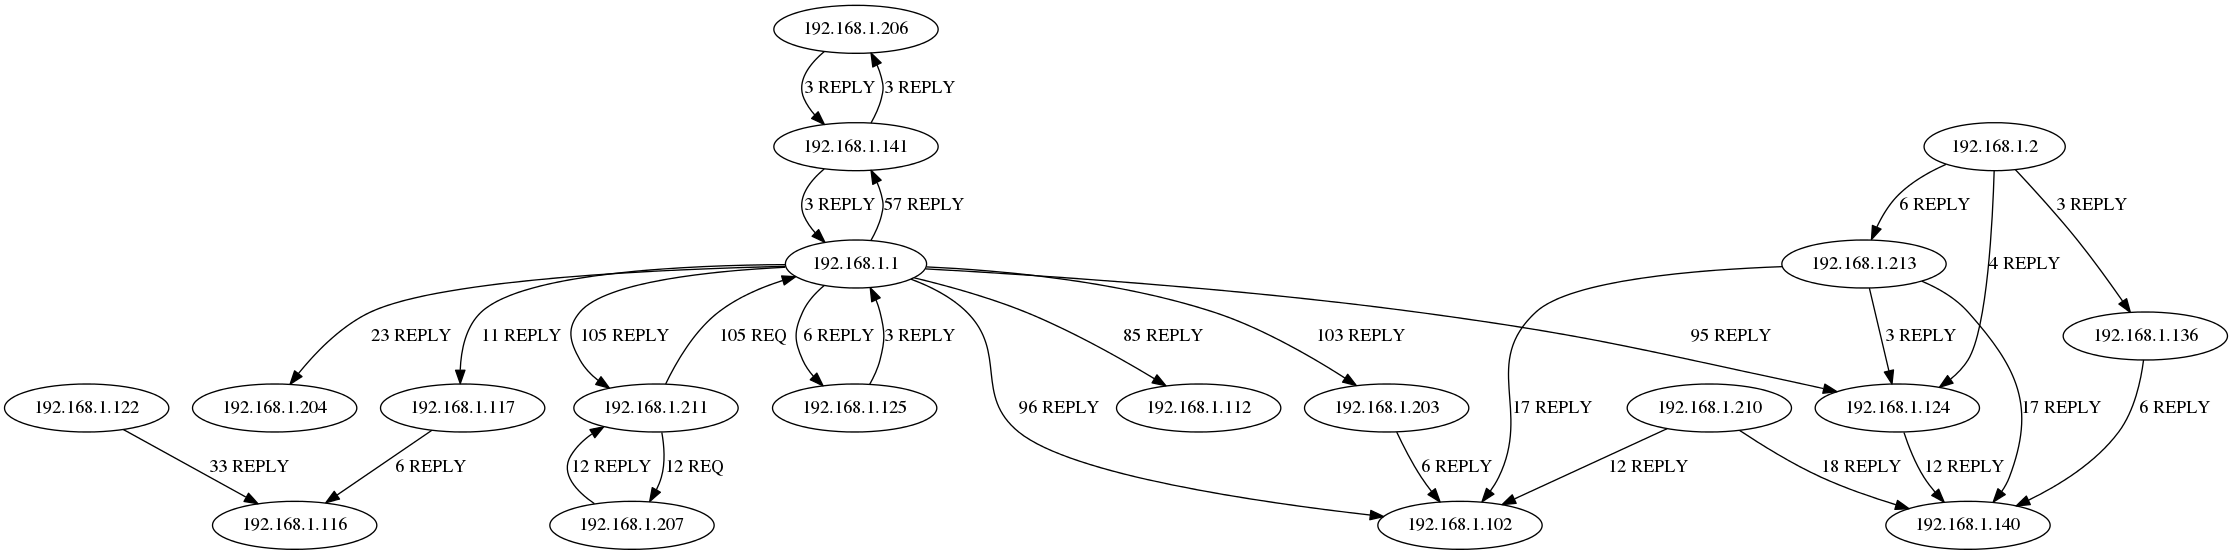
\includegraphics[angle=90, scale=0.3]{./graficos/grafos-arp/grafo_laburo_mari.png}
  \end{center}
  \caption{Digrafo: red laboral Devartis}
\end{figure}

Observando el grafo presentado, se puede notar que el nodo 192.168.1.1 es distinguido, por la cantidad de mensajes de tipo Replay que salen de mismo. Probablemente, la IP del nodo corresponda al router de la red. Esta  deducción, se podrá comprobar en el análisis de siguientes gráficos.

\subsubsection{Red Mercap}
Finalmente, la cuarta captura se realizó en el trabajo de otro de los integrantes. La red fue analizada desde una máquina virtual corriendo un sistema Linux, sobre un host Windows. Cabe aclarar que la misma estaba conectada a la red de manera física y que cuenta de 30 computadoras, 5 servidores y 1 router WiFi (además de los posibles dispositivos móviles conectados a la red de manera inalámbrica).

La captura duró una hora, durante la cual se obtuvo una enorme cantidad de relaciones generadas entre los diferentes actores, enviando y recibiendo los respectivos paquetes ARP. Esto ya aseguraba que el digrafo resultante (en primer instancia) iba a ser ilegible, aún ampliando la imagen (como observamos en el círculo con zoom sobre uno de los tantos nodos distinguidos de la red). 

Es por eso que para analizar mejor la red y la interacción por medio de paquetes, decidimos mostrar solo aquellas relaciones en las cuales se envíen o reciban mas de 20 paquetes ARP. Este filtro solo se aplica para favorecer la visualización de los datos y de ninguna manera alteramos los resultados de la captura para los experimentos posteriores. De esta manera, observamos que la presente red toma un tamaño mucho mas manejable. Limitando la cantidad de nodos a mostrar, nos podemos concentrar en ver los nodos que realmente se destacan.

A simple vista observamos que los nodos 192.168.168.1, 192.168.168.2, 192.168.168.4, 192.168.168.36 y 192.168.168.135 concentran gran parte del intercambio de mensajes ARP de este segmento de la captura. De estos nodos distinguidos, en particular podemos inferir que los que tienen IPs mas bajas, probablemente sean algunos de los servidores de los que dispone la empresa. Potencialmente, los mas antiguos y utilizados, a saber; un servidor para Envy (control de versiones orientado a objetos - Smalltalk), un servidor que aloja la web empresarial, un CVS y otras herramientas como JIRA ó BambooHR (muy consultados a toda hora), y finalmente un servidor corriendo GemStone (base de datos no relacional).

\begin{figure}{h!}{0.5\textwidth}
  \begin{center}
    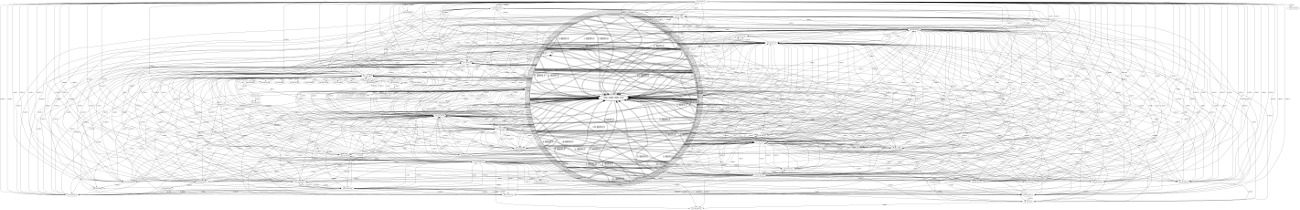
\includegraphics[angle=90,scale=0.2]{./graficos/grafos-arp/grafo_laburo_eze1.png}
  \end{center}
  \caption{Digrafo: red laboral Mercap}
\end{figure}
\newpage
\subsection{Cantidad de paquetes por cada campo Type}\label{"Type"}

A continuación, se mostrará una breve descripción de cada uno de los tipos de los paquetes Ethernet.

\underline{Protocolo ARP (Address Resolution Protocol):}

Es el protocolo encargado de encontrar la dirección MAC que corresponde a una determinada dirección IP. Para lograrlo, se envía un request ARP a la dirección de la red con MAC = FF FF FF FF FF FF, que contiene la dirección IP por la que se está preguntando. Se espera que esa máquina responda un reply ARP con la dirección IP que le corresponde.

\underline{Protocolo IP (Internet Protocol):}

Su función principal es el uso bidireccional en origen o destino de comunicación para transmitir datos mediante un protocolo no orientado a conexión que transfiere paquetes a través de distintas redes físicas.
En este protocolo no se necesita ninguna configuración antes de que un equipo intente enviar paquetes a otro con el que no se había comunicado antes.

\underline{Protocolos IPv4 (Internet Protocol version 4) y IPv6 (Internet Protocol version 6):}

IPv4 es la cuarta versión del protocolo IP, y actualmente es usada en la gran mayoría de dispositivos que acceden a Internet. IPv6 se diseñó para reemplazar a IPv4 ya que admite una mayor cantidad de direcciones de host diferentes.

\underline{Protocolo LLDP (Link Layer Discovery Protocol):}

Es utilizado por los dispositivos de la red para hacer públicos su identidad, capacidades y vecinos en una LAN IEEE 802, principalmente por cable Ethernet.
El LLDP puede ser utilizado como componente en aplicaciones de gestión de red y monitoreo.
	
\underline{LLC (Logical Link Control):}

Es la subcapa de enlace de datos responsable del control de enlace lógico. Además, maneja el control de errores, control del flujo, control de diálogo y direccionamiento de la subcapa MAC.
Los protocolos LLC son utilizados para la comunicación entre entidades de la propia subcapa LLC. También definen los procedimientos para el intercambio de tramas de información y de control entre cualquier par de puntos. 
El protocolo LLC más generalizado es IEEE 802.2.



Para cada red estudiada se presenta un gráfico con el porcentaje de paquetes tranmitidos para cada protocolo y su análisis del overhead impuesto por ARP.

\subsubsection{Red Hogareña}

\centerline{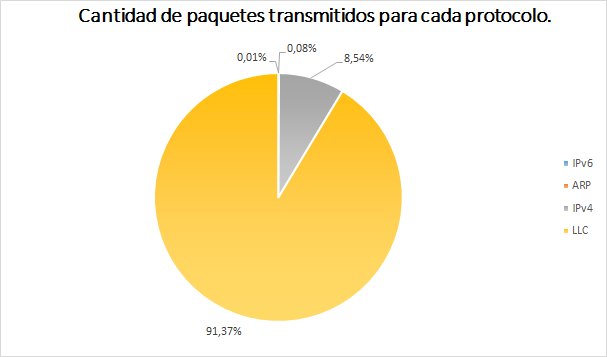
\includegraphics[width=0.8\textwidth]{./graficos/paquetesVSProtocolo/casa_mari2.png}}

Como se puede observar, la cantidad de paquetes arp es muy baja con respecto a los otros protocolos. Suponemos que se debe a que no se conectaron nuevos dispositivos y la mayoría de éstos ya eran conocidos por la red. A partir de este gráfico, se puede notar que el overhead impuesto por ARP es muy bajo.

\subsubsection{Red Laboratorio}

\centerline{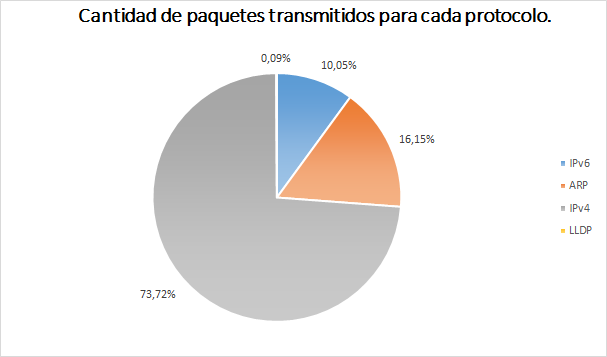
\includegraphics[width=0.8\textwidth]{./graficos/paquetesVSProtocolo/labo52.png}}
	
La sobrecarga de paquetes ARP presentada en esta red es mucho mayor a la anterior debido a que la red es mucho más grande que la anterior.

\subsubsection{Red Devartis}

\centerline{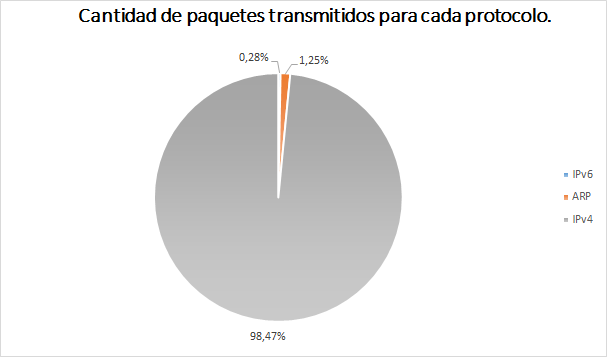
\includegraphics[width=0.8\textwidth]{./graficos/paquetesVSProtocolo/laburo_mari2.png}}

\subsubsection{Red Mercap}

\centerline{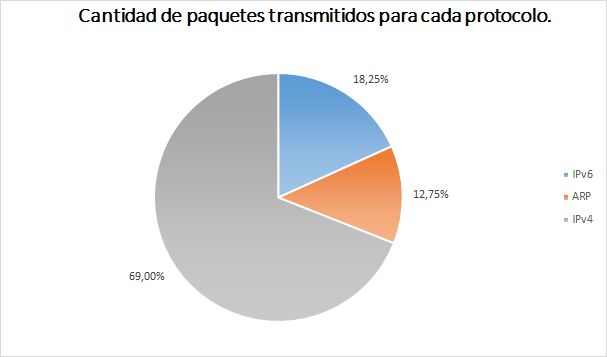
\includegraphics[width=0.8\textwidth]{./graficos/paquetesVSProtocolo/laburo_eze2.png}}


Analizando los gráficos obtenidos a partir de cada red, se puede notar que el porcentaje de paquetes ARP con respecto al resto de los protocolos es bajo. Comparándolos entre sí, se puede apreciar que cuanto más grande es la red mayor es el overhead impuesto por ARP.

Podemos agregar que el overhead afeta al throughput (cantidad de datos que se entregan por unidad de tiempo) de una conexión. Esto se debe que hay un "desperdicio" de ancho de banda, causado por la información adicional (control, secuencia, etc) que debe viajar en los paquetes además de los datos, ya que estos datos extra no contribuyen al contenido del mensaje.
\newpage
\subsection{Entropía de acuerdo al tiempo transcurrido}

\subsubsection{Red Hogareña}


\centerline{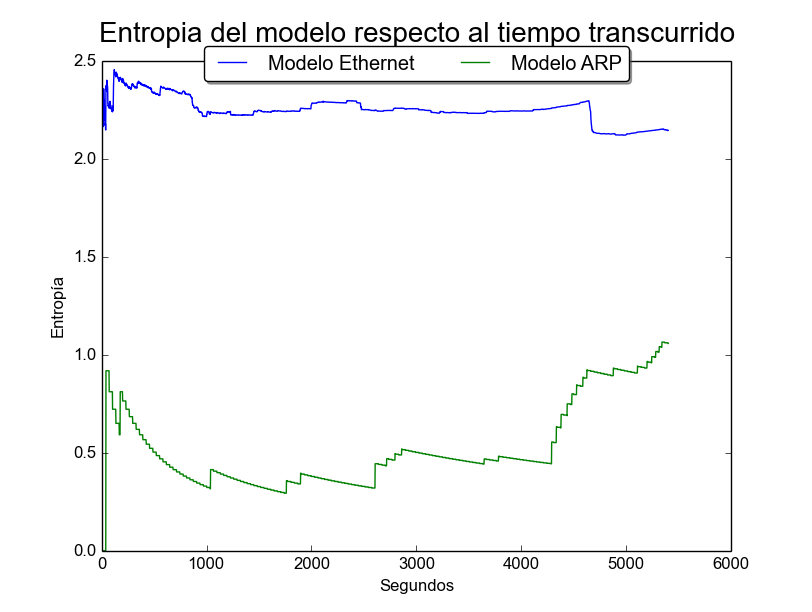
\includegraphics[width=0.8\textwidth]{./graficos/entrophyVSTime/casa_mari.png}}


\subsubsection{Red Laboratorio}


\centerline{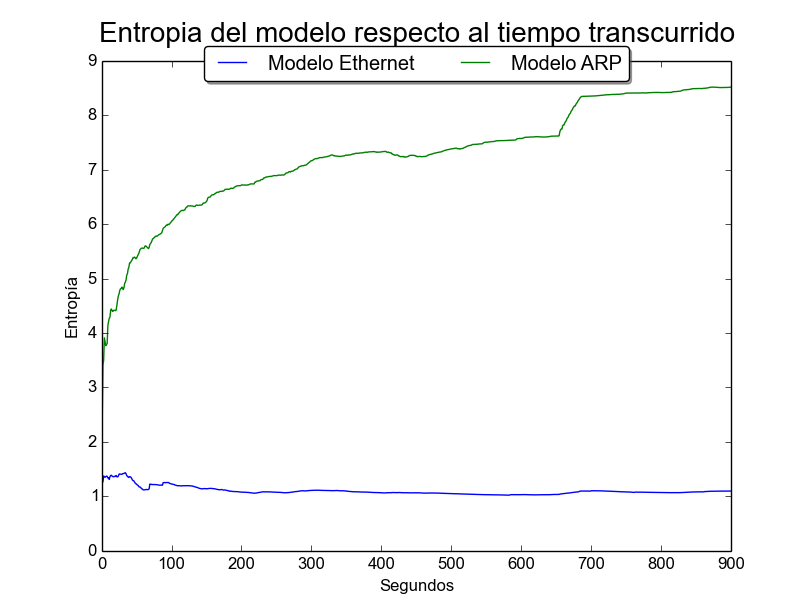
\includegraphics[width=0.8\textwidth]{./graficos/entrophyVSTime/labo5.png}}


\newpage
\subsubsection{Red Devartis}


\centerline{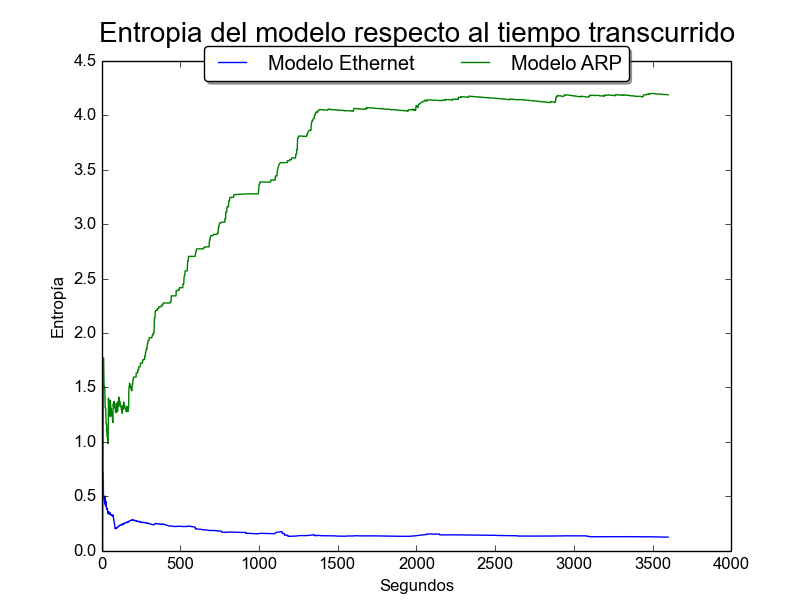
\includegraphics[width=0.8\textwidth]{./graficos/entrophyVSTime/laburo_mari.png}}


\subsubsection{Red Mercap}


\centerline{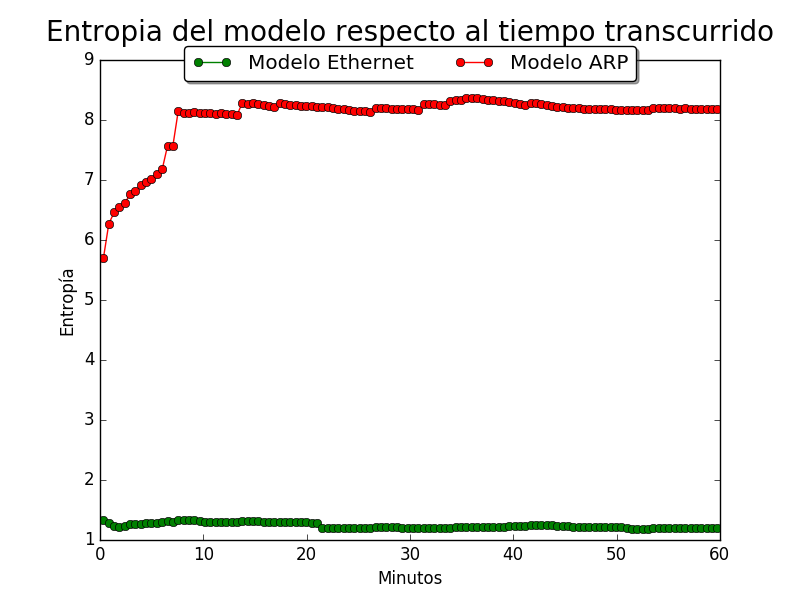
\includegraphics[width=0.8\textwidth]{./graficos/entrophyVSTime/laburo_eze.png}}
\newpage
\section{Conclusiones}

\newpage

\section{Utilización de la herramienta de captura}

Para realizar la captura de paquetes, se implementó una herramienta en Python. Para poder utilizar la misma se debe tener instalados los siguientes paquetes:

\begin{itemize}
	\item python 2.7
	\item pyqt4 (para python 2.7)
	\item scapy
\end{itemize}

Para ejecutar la aplicación se debe ejecutar el siguiente comando en consola:

\begin{figure}[h!]
	\centering
	\begin{lstlisting}
	[ignacio@desktop ~]$ sudo ./arp
	\end{lstlisting}
\end{figure}

o:


\begin{figure}[h!]
	\centering
	\begin{lstlisting}
	[ignacio@desktop ~]$ sudo python2 arp
	\end{lstlisting}
\end{figure}

El archivo \emph{arp} se encuentra dentro de la carpeta que contiene la herramienta.

\begin{figure}[h!]
	\caption{Herramienta de Captura, pantalla principal.}
	\centering
	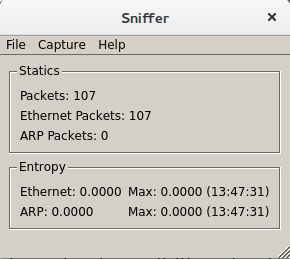
\includegraphics[width=0.25\textwidth]{graficos/tool/tool}
\end{figure}

Para comenzar una nueva captura, se debe elegir la opción \emph{Start} del menú \emph{Capture}. Para detener la misma seleccionar la opción \emph{Stop} del mismo menú.

% mostrar menú (no le puedo sacar una foto... WTF?!)

También la aplicación da la opción de realizar capturas por intervalos de tiempo en minutos. Para activarla, seleccionar \emph{Interval} del menú \emph{Capture}.

\begin{figure}[h!]
        \centering
        \begin{subfigure}[b]{0.3\textwidth}
                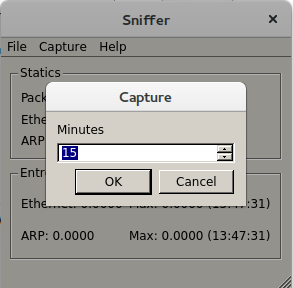
\includegraphics[width=\textwidth]{graficos/tool/tool_interval}
                \caption{Duración de la captura}
        \end{subfigure}%
        ~ %add desired spacing between images, e. g. ~, \quad, \qquad, \hfill etc.
          %(or a blank line to force the subfigure onto a new line)
        \begin{subfigure}[b]{0.3\textwidth}
                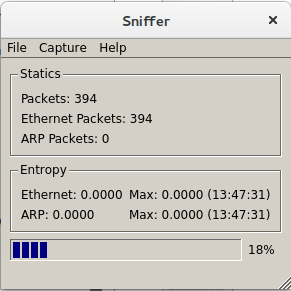
\includegraphics[width=\textwidth]{graficos/tool/tool_progress}
                \caption{Evolución de la captura}
        \end{subfigure}
        ~ %add desired spacing between images, e. g. ~, \quad, \qquad, \hfill etc.
          %(or a blank line to force the subfigure onto a new line)
        \begin{subfigure}[b]{0.3\textwidth}
                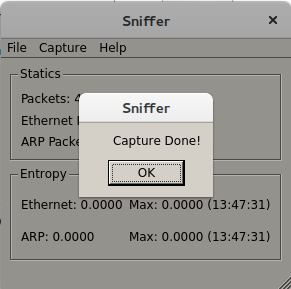
\includegraphics[width=\textwidth]{graficos/tool/tool_done}
                \caption{Captura terminada}
        \end{subfigure}
        \caption{Capturando durante un intervalo de tiempo en minutos.}\label{fig:interval}
\end{figure}

\newpage

Para almacenar la información capturada por la herramienta, la misma posee dos opciones bajo el menú \emph{File}. Dichas opciones son:

\begin{description}
	\item[Save Capture]	Guarda los paquetes capturados dentro de un archivo de texto plano.
	\item[Save Entropy] A cada segundo la herramienta calcula la entropía de ambas fuentes. Esta opción salva dicha información en un archivo de texto plano.
\end{description}


\end{document}
